\section{Montaje}

Para la construcción del nodo 2, usaremos el siguiente cableado de la placa
Arduino Pro Mini:

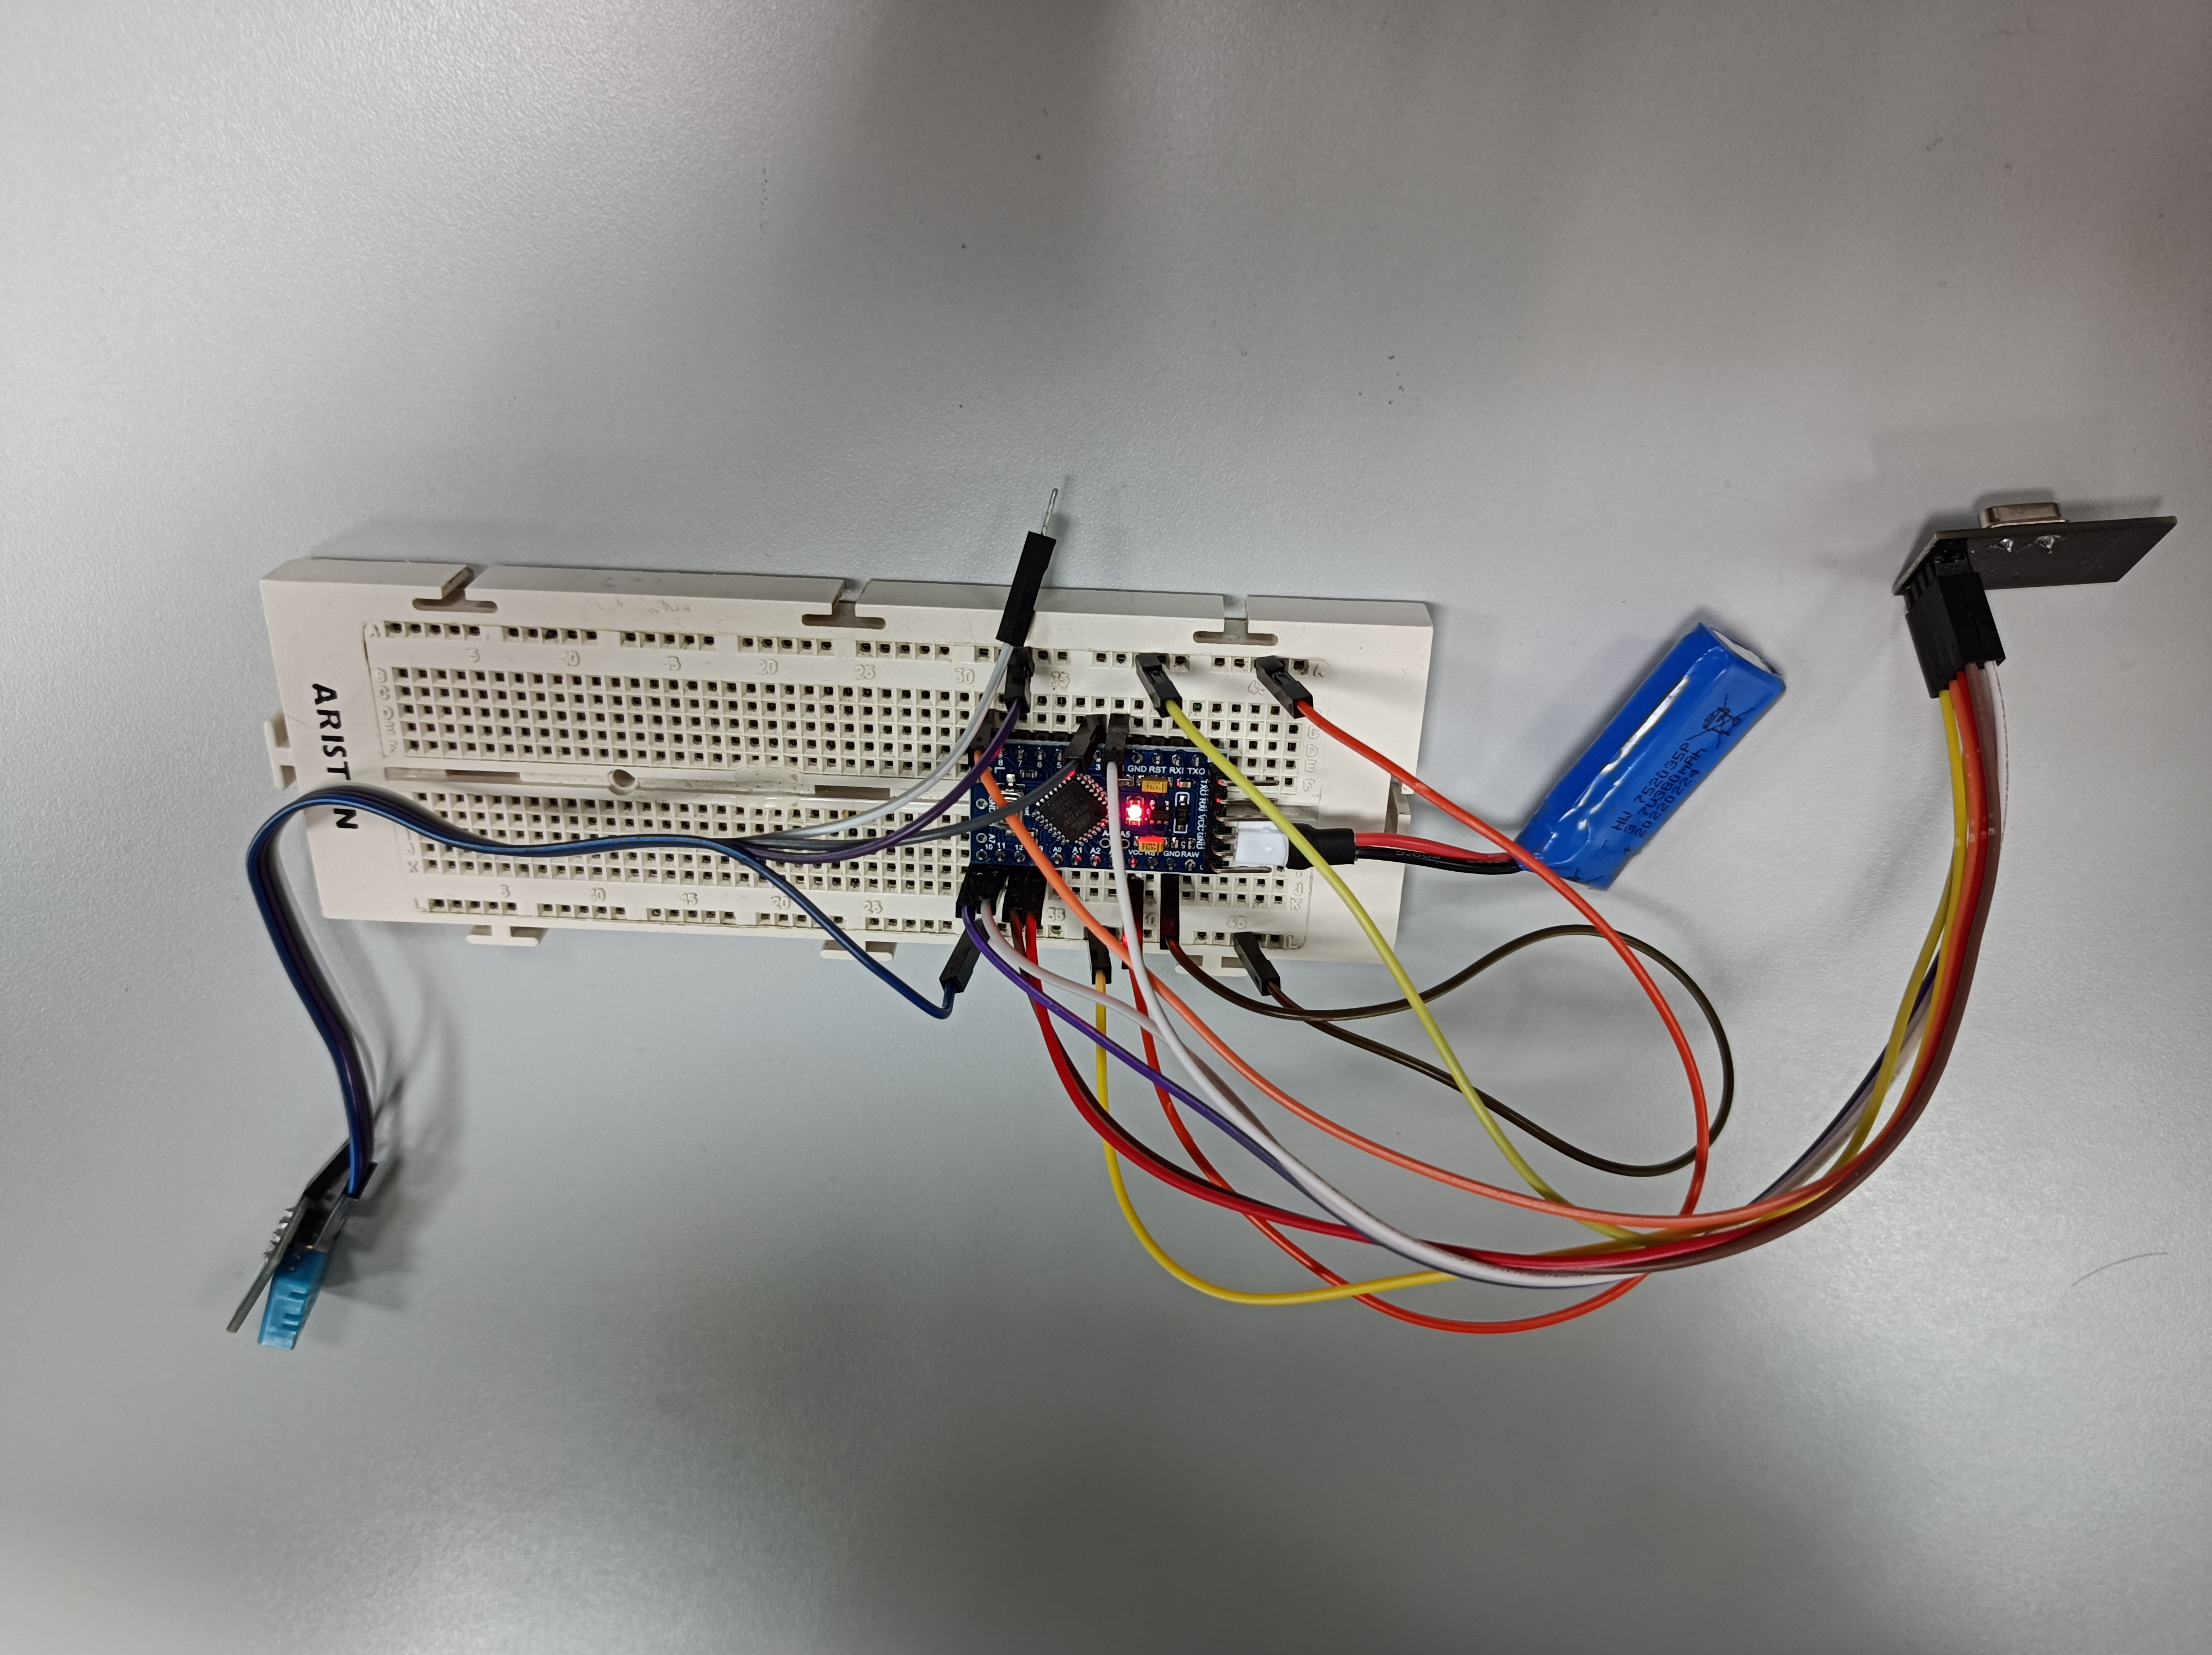
\includegraphics[width=\linewidth]{nodo2/nodo2-wiring.jpg}

Para la programación de la placa, además de la librería \emph{MySensors},
necesitamos las librerías \emph{arduino-DHT}\footnote{\url{
    https://github.com/markruys/arduino-DHT/archive/cd24ce3ca32fe0caf05d6c21565c8d5605860a08.zip
}} y \emph{Arduino\_Vcc}\footnote{\url{
    https://github.com/Yveaux/Arduino_Vcc/archive/2b2362b52e79ce102088c690e2bbcc595563c859.zip
}}.

Usaremos este código:

\lstinputlisting[language=C++, caption=nodo2.ino]{2/nodo2/nodo2.ino}

En este caso, en el menú \emph{Configuración $\rightarrow$ Dispositivos}
debería salir una entrada con las lecturas de temperatura y humedad combinadas,
y la del nivel de batería. También saldrá una lectura adicional de temperatura
que no indica ningún valor, esto es un comportamiento extraño de Domoticz en la
comunicación con MySensors que se desconoce por qué lo hace:

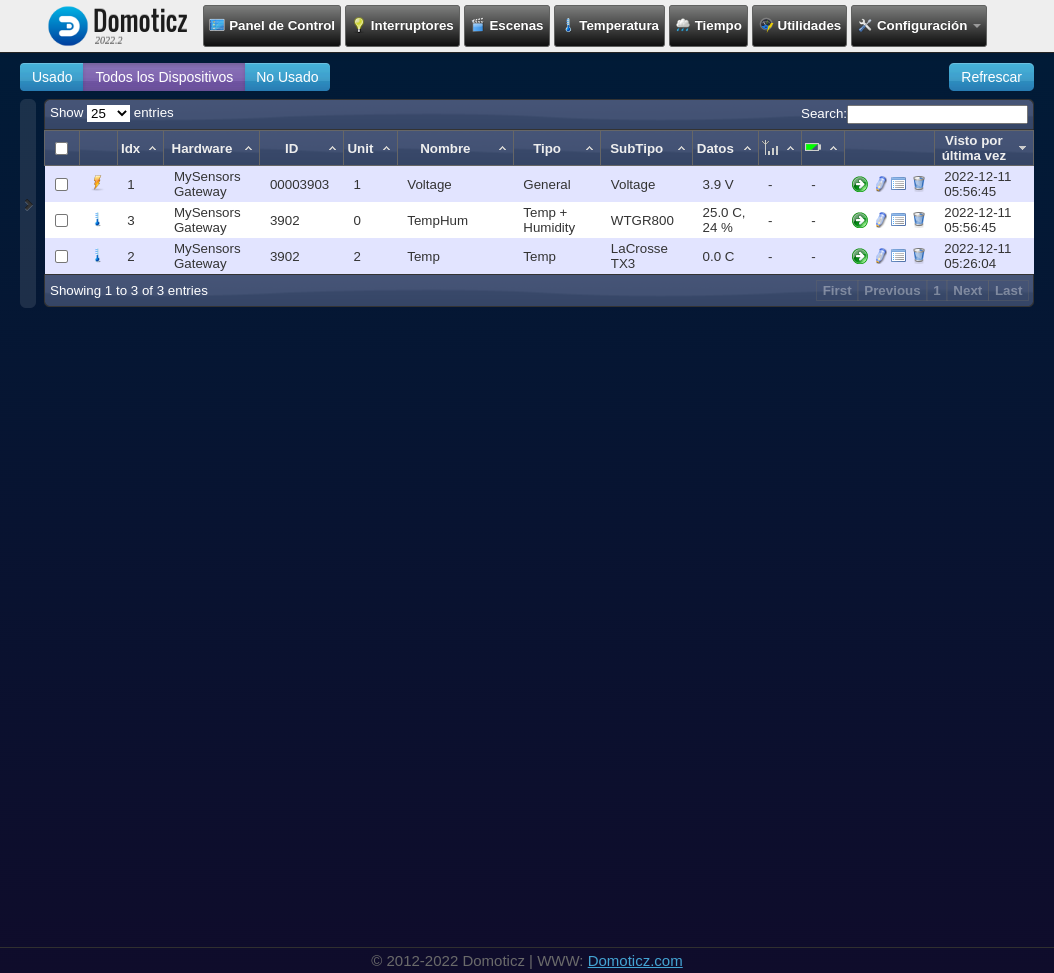
\includegraphics[width=\linewidth]{nodo2/nodo2-domoticz.png}

\section{Medición del consumo}

Para medir el consumo del sistema mientras opera realizaremos el siguiente
montaje. Nótese que la polaridad de la conexión del medidor es la inversa de la
recomendada en el enunciado de la práctica. Esto se hace para evitar lecturas
negativas de intensidad.

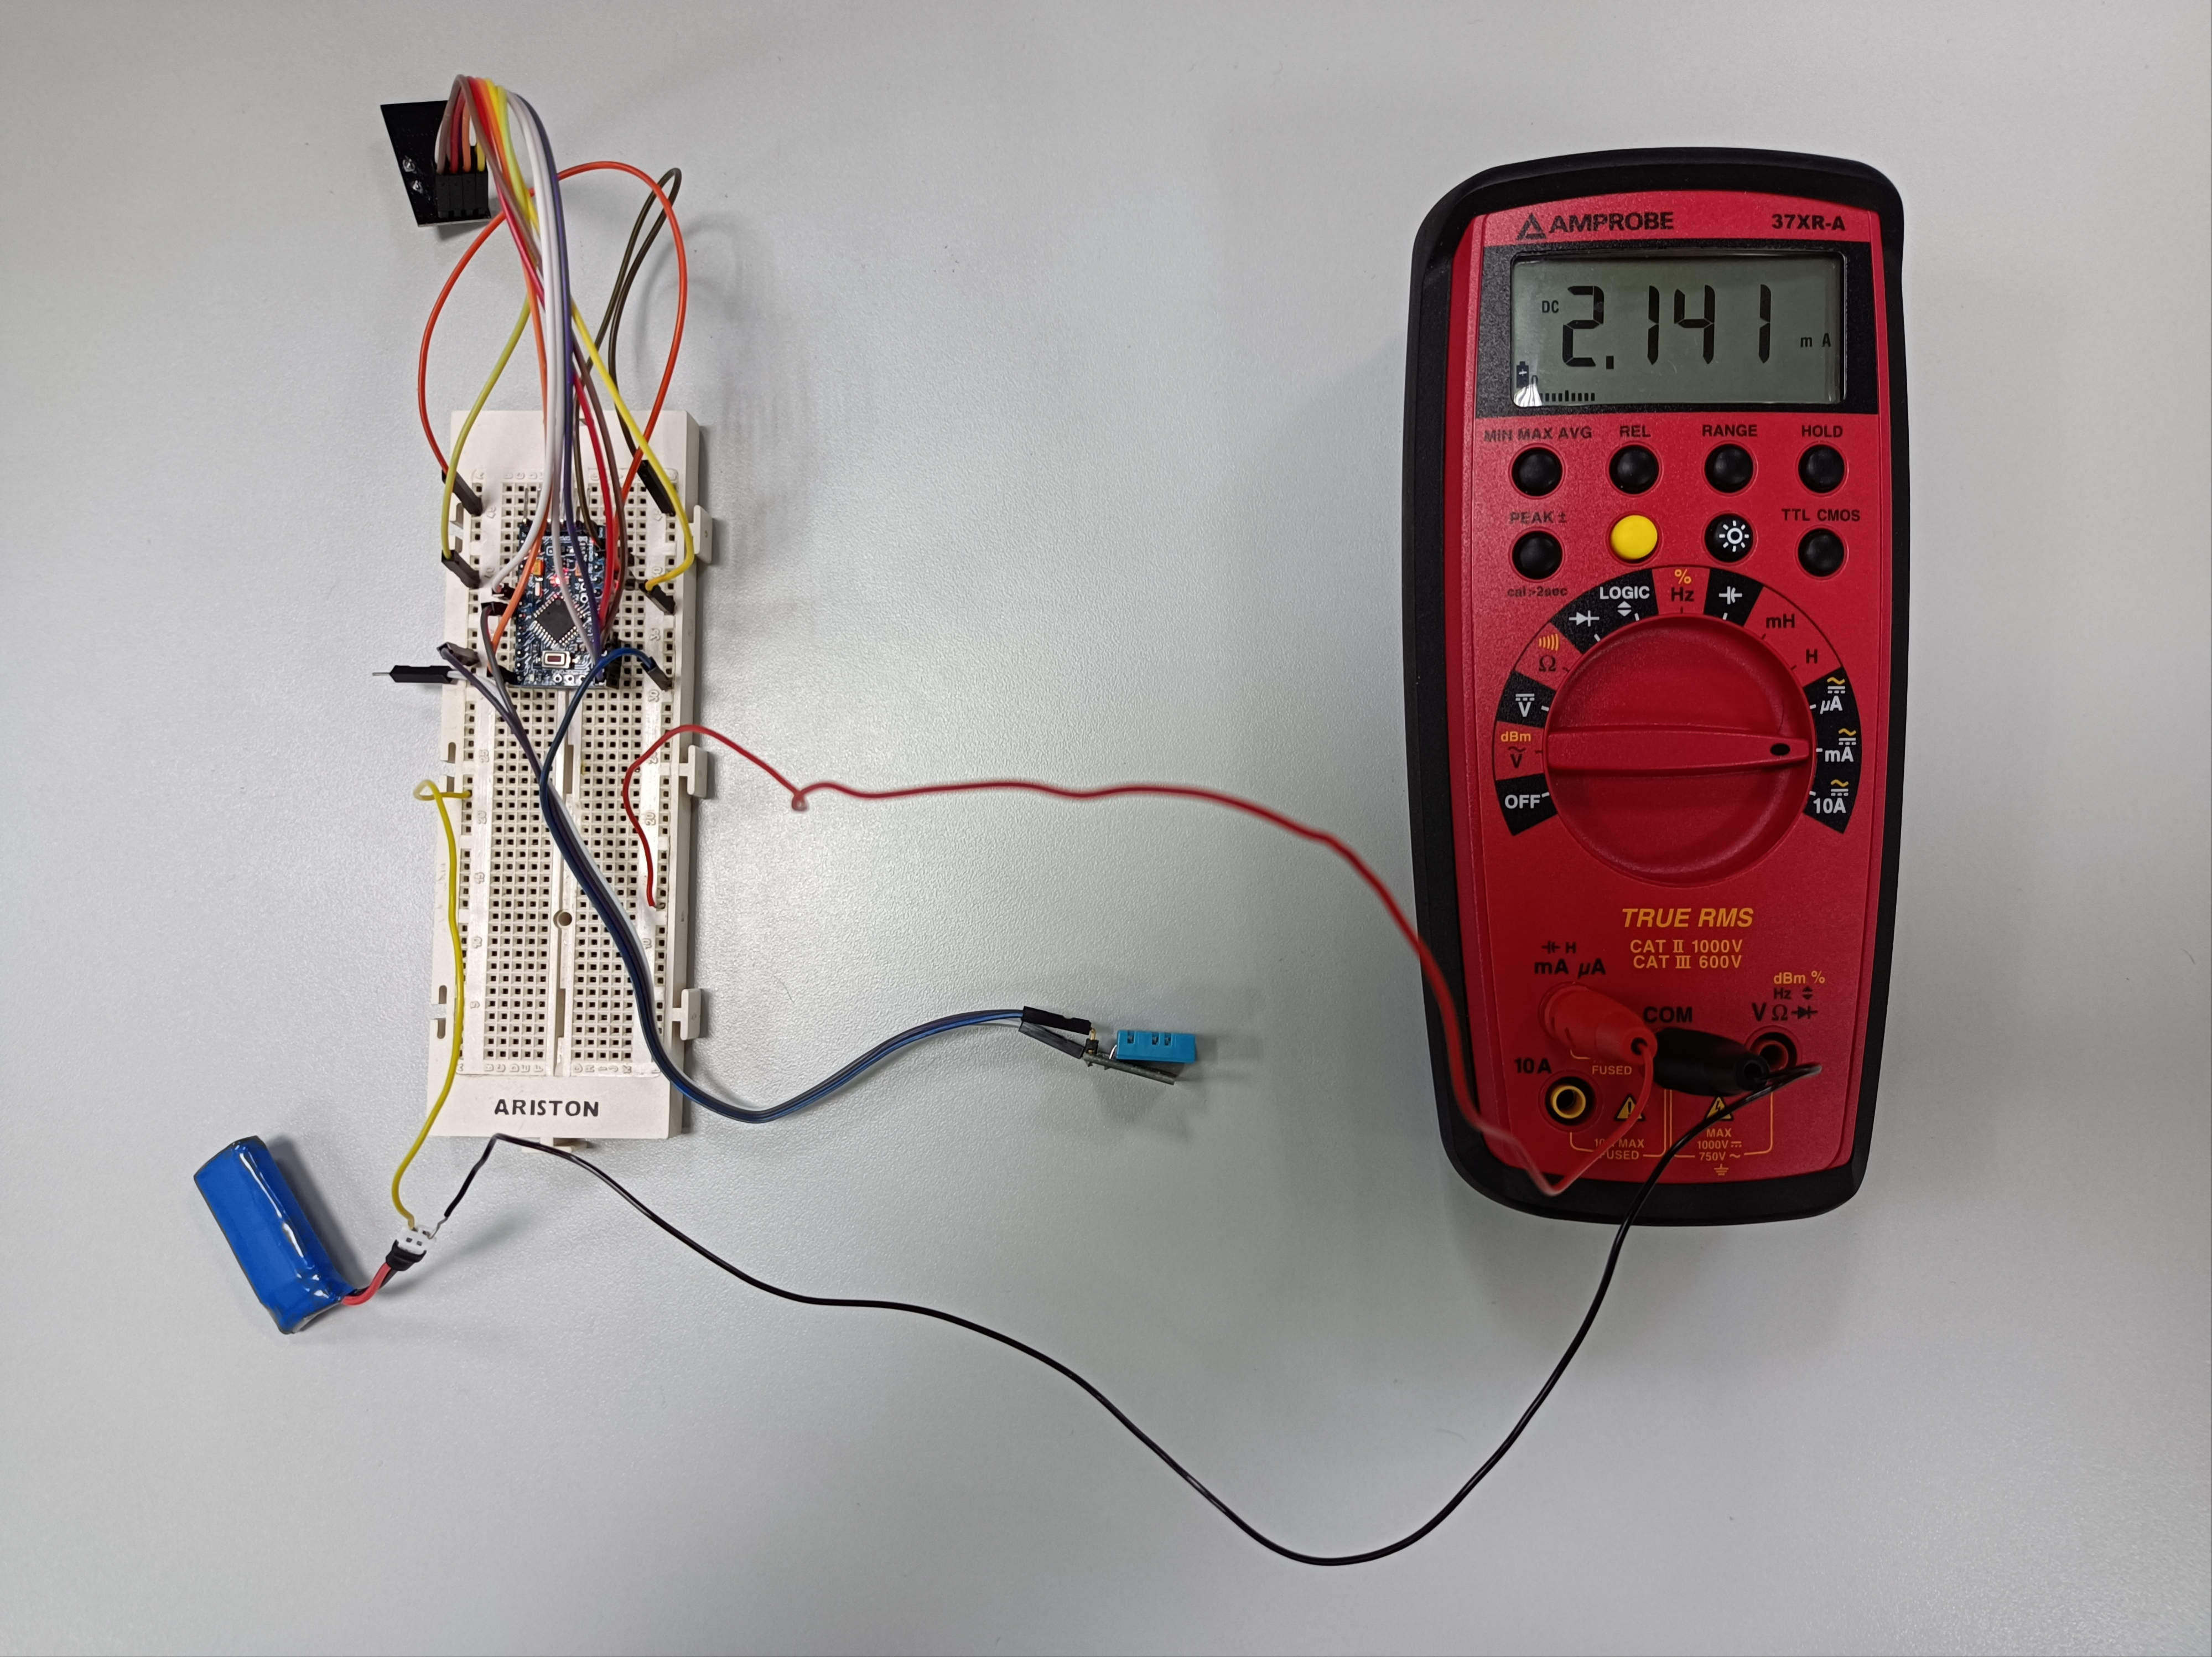
\includegraphics[width=\linewidth]{nodo2/nodo2-consumption.jpg}

La intensidad eléctrica que muestra el medidor es la correspondiente a la
espera entre transmisiones de los valores de medida. Cuando se transmiten datos
este consumo es aproximadamente el doble. Teniendo en cuenta que la tensión de
la batería utilizada era de 3.9 V, entonces el consumo de potencia era de
$2.141\ mA \cdot 3.9\ V \approx 8.35 mW$.

Se sabe que una parte significativa de este consumo base de operación es por el
regulador de tensión incorporado, aunque no se ha realizado la prueba con otra
placa que no lo integre para cuantificar con precisión su impacto.